\part{Memory Management}

\chapter{Subsystem Overview}

This chapter briefly introduces the architectural layout of memory management
in Zeke at very generic level. Specifically we do not cover memory map layout or
anything hardware specific things here.

Zeke as well as most of major operating systems does its memory management and
mapping in multiple stages. In the kernel stages are built into following layers
of abstraction \ac{MMU} abstraction, \verb+dynmem+ handling dynamic allocation
of contiguous blocks of memory and \verb+kmalloc+ that allocates memory for the
kernel itself. These are the most important parts of the memory management in
Zeke as other parts of the kernel are only utilizing these to allocate or map
memory for use anywhere in the system.

Figure \ref{figure:mm_layers} shows the memory management stack from
top to bottom.

\begin{figure}
  \begin{tikzpicture}
  [node distance=.8cm,
  start chain=going below,]
  	%\node[punktchain, join] (vfs)     {vfs};
	%\node[punktchain, join] (ramfs)   {ramfs};
    %\begin{scope}[start branch=ofsb]
   	%	\node[punktchain, on chain=going right] (ofs) {some other FS};
    %\end{scope}
    \node[punktchain, join] (kmalloc) {kmalloc};
    \node[punktchain, join] (dynmem)  {dynmem};
    \node[punktchain, join] (mmu)     {mmu HAL};
    \node[punktchain, join] (cpusp)   {CPU specific code};
    \node[punktchain, join] (hw)      {MMU \& coProcessor};
    %
    %\draw[|-,-|,->, thick,] (vfs.south) |-+(0,-1em)-| (ofs.north);
  % Now, let us add some braches. 
  %\draw[tuborg, decoration={brace}] let \p1=(ramfs.north), \p2=(kmalloc.south) in
  %  ($(2, \y1)$) -- ($(2, \y2)$) node[tubnode] {Scope of this document.};
  \end{tikzpicture}
  \centering
  \caption{Kernel layers from kmalloc to physical \acs{CPU} level.}
  \label{figure:mm_layers}
\end{figure}

\begin{description}
\item[kmalloc] is a malloc-like interface for allocating arbitrary sized blocks
  of memory.
\item[dynmem] is a block allocator that always allocates memory in block size of
  $1 \:\textrm{MB}$. See fig. \ref{figure:dynmem_blocks}.
\end{description}

Lets assume that some part of the kernel needs a new chunk of memory for some
temporal use, there is no more space left at any of the higher levels and most
importantly the code uses \verb+kmalloc+ to allocate the block. What happens
next is that memory allocation request is eventually passed to dynmem memory
allocator.

dynmem tries to locate the first free memory region in the dynmem memory section
that satisfies the condition
$\textrm{requested size} \le n \times 1 \:\textrm{MB}$. If dynmem finds a free
region it is then reserved and returned to \verb+kmalloc+. \verb+kmalloc+ will
then allocate memory from that and possibly other closely located reservations
for the original caller by using its own algorithm, which is at the moment quite
naive first fit algorithm.

kmalloc stores its linked list of reserved and free blocks in the same memory
that is used to allocate memory for its clients. Listing \ref{list:mblockt}
showsthe \verb+mblock_t+ structure definition used internally in kmalloc for
linking blocks of memory.

\begin{figure}
  \newcommand{\colorbitbox}[3]{%
\rlap{\bitbox{#2}{\color{#1}\rule{\width}{\height}}}%
\bitbox{#2}{#3}}

\definecolor{lightgreen}{rgb}{0.64,1,0.71}
\definecolor{lightred}{rgb}{1,0.7,0.71}

\begin{bytefield}[boxformatting={\centering\small},bitwidth=\widthof{Kernel~}]{4}
  \bitheader[endianness=little]{0-3} \\
  \colorbitbox{lightred}{1}{Kernel} &
  \colorbitbox{lightgreen}{1}{} &
  \colorbitbox{lightred}{2}{User} &
\end{bytefield}
  \centering
  \caption{Example of reserved dynmem regions.}
  \label{figure:dynmem_blocks}
\end{figure}

\lstinputlisting[label=list:mblockt,caption=kmalloc mblock\_t struct definition.]{mem/mblock_t.c}


\chapter{Virtual Memory}

\section{Introduction to vmem in Zeke}

Every process has its own master page table and varying number of L2 page
tables. Kernel has its own master page table too. Static/fixed entries are
copied to all master page tables created. Process shares its master page
table with its childs.

Process page tables are stored in dynmem area.

ARM note: Only 4 kB pages are used with L2 page tables so XN (Execute-Never) bit
is always usable also for L2 pages.

\subsection{Domains}

See \verb+MMU_DOM_xxx+ definitions.

\subsection{Virtual memory abstraction levels}

\begin{figure}
\begin{verbatim}
U                      +---------------+
S                      |    malloc     |
R                      +---------------+
-------------------------------|-----------------
K   +---------------+  +---------------+
E   |    kmalloc    |  |    process    |
R   +---------------+  +---------------+
N           |     /\    |      |
E           |     |    \/      |
L           |  +--------+   +----+
            |  |vralloc |---| vm |
            |  +--------+   +----+
            |     |            |
           \/    \/           \/
    +---------------+     +----------+
    |    dynmem     |-----| ptmapper |
    +---------------+     +----------+
            |                  |
           \/                  |
    +---------------+          |
    |    mmu HAL    |<----------
    +---------------+
            |
    +-----------------------+
    | CPU specific MMU code |
    +-----------------------+
------------|------------------------------------
    +-------------------+
    | MMU & coProcessor |
    +-------------------+
\end{verbatim}
\caption{Virtual memory related subsystems in Zeke.}
\label{figure:vmsubsys}
\end{figure}

See figure \ref{figure:vmsubsys}.

\begin{itemize}
  \item \verb+kmalloc+  - is a kernel level memory allocation service, used
                        solely for memory allocations in kernel space.
  \item \verb+vralloc+  - VRAlloc is a special memory allocator targetted to
                        allocate blocks of memory that will be mapped in virtual
                        address space of processes, it returns \verb+vm_region+
                        structs instead of just base address of the allocation.
  \item \verb+dynmem+   - is a dynamic memory allocation system that allocates
                        \& frees contiguous blocks of physical memory.
  \item \verb+ptmapper+ - owns the statically created page tables (particularly
                        the master page table) and regions, and is also used to
                        allocate new page tables from the page table region.
  \item \verb+vm+       - vm runs various checks on virtual memory access,
                        copies data between user land and kernel space and
                        allocates memory for processes.
  \item mmu HAL -       is the abract MMU interface provided by \verb+mmu.h+
                        and \verb+mmu.c+.
  \item CPU specific MMU code is the module responsible of configuring the
        physical MMU layer and implementing the interface prodived by
        \verb+mmu.c+
\end{itemize}


\chapter{kmalloc}

The current implementation of a generic kernel memory allocator is largely
based on a tutorial written by Marwan Burrelle\cite{Burelle:malloc}.

\section{Brief Description}

The current kernel memory allocator implementation is somewhat naive and
exploits some very simple techniques like the first fit algorithm for allocating
memory.

The idea of the first fit algorithm is to find a first large enough free block
of memory from an already allocated region of memory. This is done by traversing
the list of memory blocks and looking for a sufficiently large block. This is
of course quite sub-optimal and better solutions has to be considered in the
future. When a large enough block is found it's split in two halves so that the
left one corresponds to requested size and the right block is left free. All data
blocks are aligned to 4 byte access.

Fragmentation of memory blocks is kept minimal by immediately merging newly freed
block with neighboring blocks. This approach will keep all free blocks between
reserved blocks contiguous but it doesn't work if there is lot of allocations of
different sizes that are freed independently. Therefore the current implementation
will definitely suffer some fragmentation over time.

When kmalloc is out of (large enough) memory blocks it will expand its memory
space by allocating a new block of memory from dynmem. Allocation is commited in
1 MB blocks (naturally) and always rounded to the next 1 MB.

\begin{figure}
\begin{verbatim}
    +-+------+-+---------+-+-------+
    |d|      |d|         |d|       |
    |e| DATA |e|  FREE   |e| DATA  |
    |s|      |s|         |s|       |
    |c|      |c|         |c|       |
    +-+------+-+---------+-+-------+
\end{verbatim}
\caption{Kmalloc blocks.}
\label{figure:kmalloc_blocks}
\end{figure}

Descriptor structs are used to store the size of the data block, reference counters,
and pointers to neighbouring block descriptors.


\section{Suggestions for Further Development}

\subsection{Memory allocation algorithms}

The current implementation of kmalloc relies on first-fit algorithm and variable
sized blocks, that are processed as a linked list, which is obviously inefficient.

One achievable improvement could be adding a second data structure that would
maintain information about free memory blocks that could be used to store the
most common object sizes. This data structure could be also used to implement
something like best-fit instead of first-fit and possibly with even smaller
time complexity than the current implementation.

\begin{eqnarray}
\mathrm{proposed\_size} &=& \mathrm{req\_size}
  + \frac{\mathrm{curr\_size}}{\mathrm{req\_size}} \mathrm{o\_fact}
  + \frac{\mathrm{curr\_size}}{o\_div}.
\end{eqnarray}

\begin{algorithm}
  \caption{krealloc over commit}
  \label{algo:realloc_oc}
  \begin{algorithmic}
      \If{$\mathrm{req\_size} > \mathrm{proposed\_size}$}
        \State $\mathrm{new\_size} \gets \mathrm{req\_size}$
      \Else
        \If{$\mathrm{limit}_{min} < 4 \frac{proposed\_size}{req\_size} < \mathrm{limit}_{max}$}
          \State $\mathrm{new\_size} \gets \mathrm{proposed\_size}$
        \Else
          \State $\mathrm{new\_size} \gets \mathrm{max(req\_size, curr\_size})$
        \EndIf
      \EndIf
  \end{algorithmic}
\end{algorithm}

Figure \ref{figure:realloc} shows "simulations" for a over committing realloc
function. This is however completely untested and intuitively derived method
but it seems to perform sufficiently well for hypothetical memory allocations.

\begin{figure}
  \center
  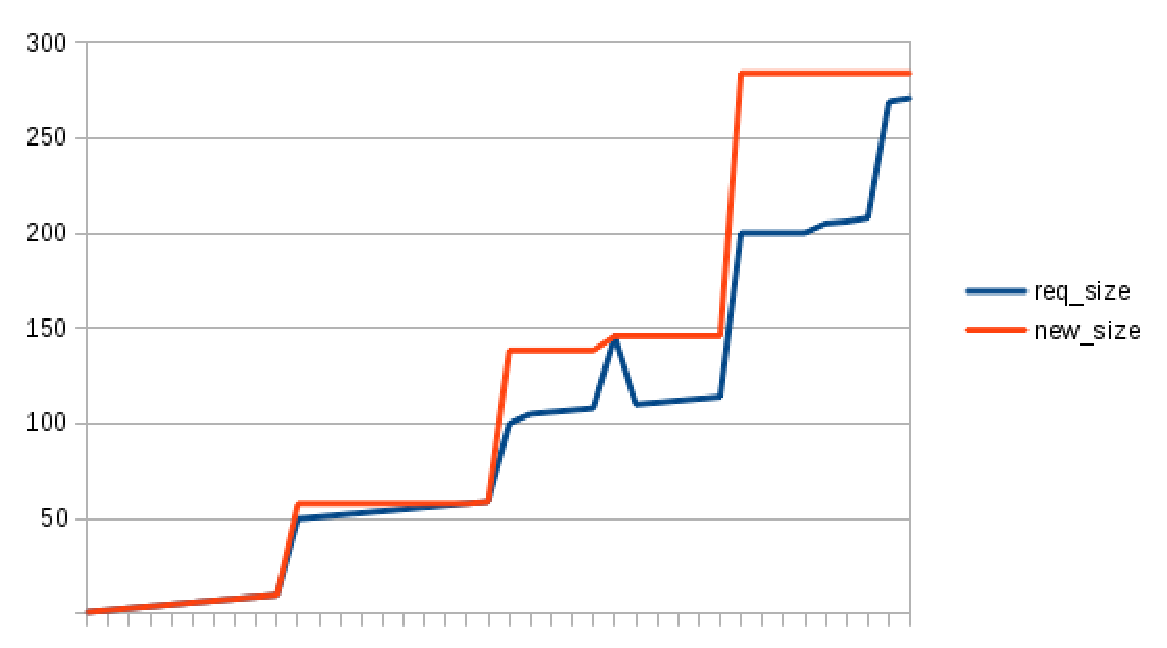
\includegraphics[width=10cm]{pics/realloc}
  \caption{New realloc method.}
  \label{figure:realloc}
\end{figure}

